\section{Software Maintenance for Large-Scale Systems}

Since an already built large-scale software system is quite complex, understanding this system requires certain strategies and tools. When a problem arises in complex software architectures, such as microservices or service-oriented architectures, resolving it often demands significant resources. These architectures consist of numerous interconnected components, and identifying the root cause of an issue can be challenging. The process may involve extensive debugging, analyzing logs, coordinating between multiple teams, and sometimes even re-evaluating design decisions. This can result in considerable time, effort, and cost being spent to restore functionality and ensure the system operates smoothly. The post-development usability issues in software systems sometimes require significant architectural changes~\citep{Folmer2005}. In order to deal with such architectural changes, an understanding of the whole system is required, and if the system is large enough, major resources are spent fixing even minor issues.

 Multiple surveys indicate that software maintenance consumes 60\% to 80\% of the total life cycle costs. Also, the maintenance costs are largely due to enhancement (often 75{-}80\%), rather than corrections~\citep{SeMaintainance2001}. To address these challenges, there is a growing need for tools that can assist in resolving bugs and reducing maintenance overhead. Such tools should be capable of reverse engineering software systems to provide a clear and comprehensive view of the architecture. By highlighting the key components and their interactions, these tools make it easier for developers to understand the system, identify issues, and perform necessary tasks efficiently. This not only simplifies debugging but also enhances the overall maintainability of the software, ensuring smoother operation and reduced downtime.

\begin{figure}[H]
    \centering
    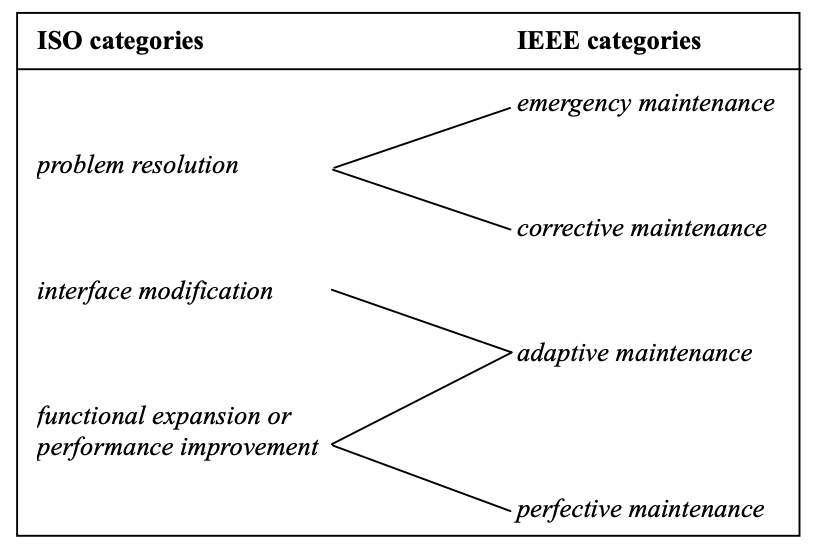
\includegraphics[width=0.8\textwidth]{figures/maintenance_process.png}
    \caption[ISO and IEEE maintenance categories]{ISO and IEEE maintenance categories (adapted from~\cite{SeMaintainance2001})}
	\label{fig_se_maintenance}
\end{figure}